\myChapter{Architectures}
\label{chap:Architectures}

In this chapter, we will provide an overview of the architectures of the UNet and SRUNet models that were utilized in our experiments. Furthermore, we will outline the training setup that we employed, which involves a Generative Adversarial Network (GAN) framework with a combination of LPIPS and SSIM as the generator loss.

\section{UNet Architecture}

The UNet architecture was introduced by Ronneberger et al. \cite{ronneberger2015u} in 2015 for biomedical image segmentation tasks. Since then, it has been widely used for various image processing tasks, including super-resolution.

The UNet architecture consists of a contracting path and an expanding path. The contracting path is composed of a series of convolutional layers with max pooling layers in between. This path downsamples the input image to a lower resolution, while increasing the number of channels. The expanding path then upsamples the low-resolution feature map back to the original size of the input image, while decreasing the number of channels.

The expanding path also has skip connections that connect the corresponding feature maps from the contracting path to the expanding path. These skip connections help the model to preserve high-frequency information from the original input image.

\Cref{fig:unet} shows an high-level representation of the UNet architecture.

\begin{figure}[h]
\centering
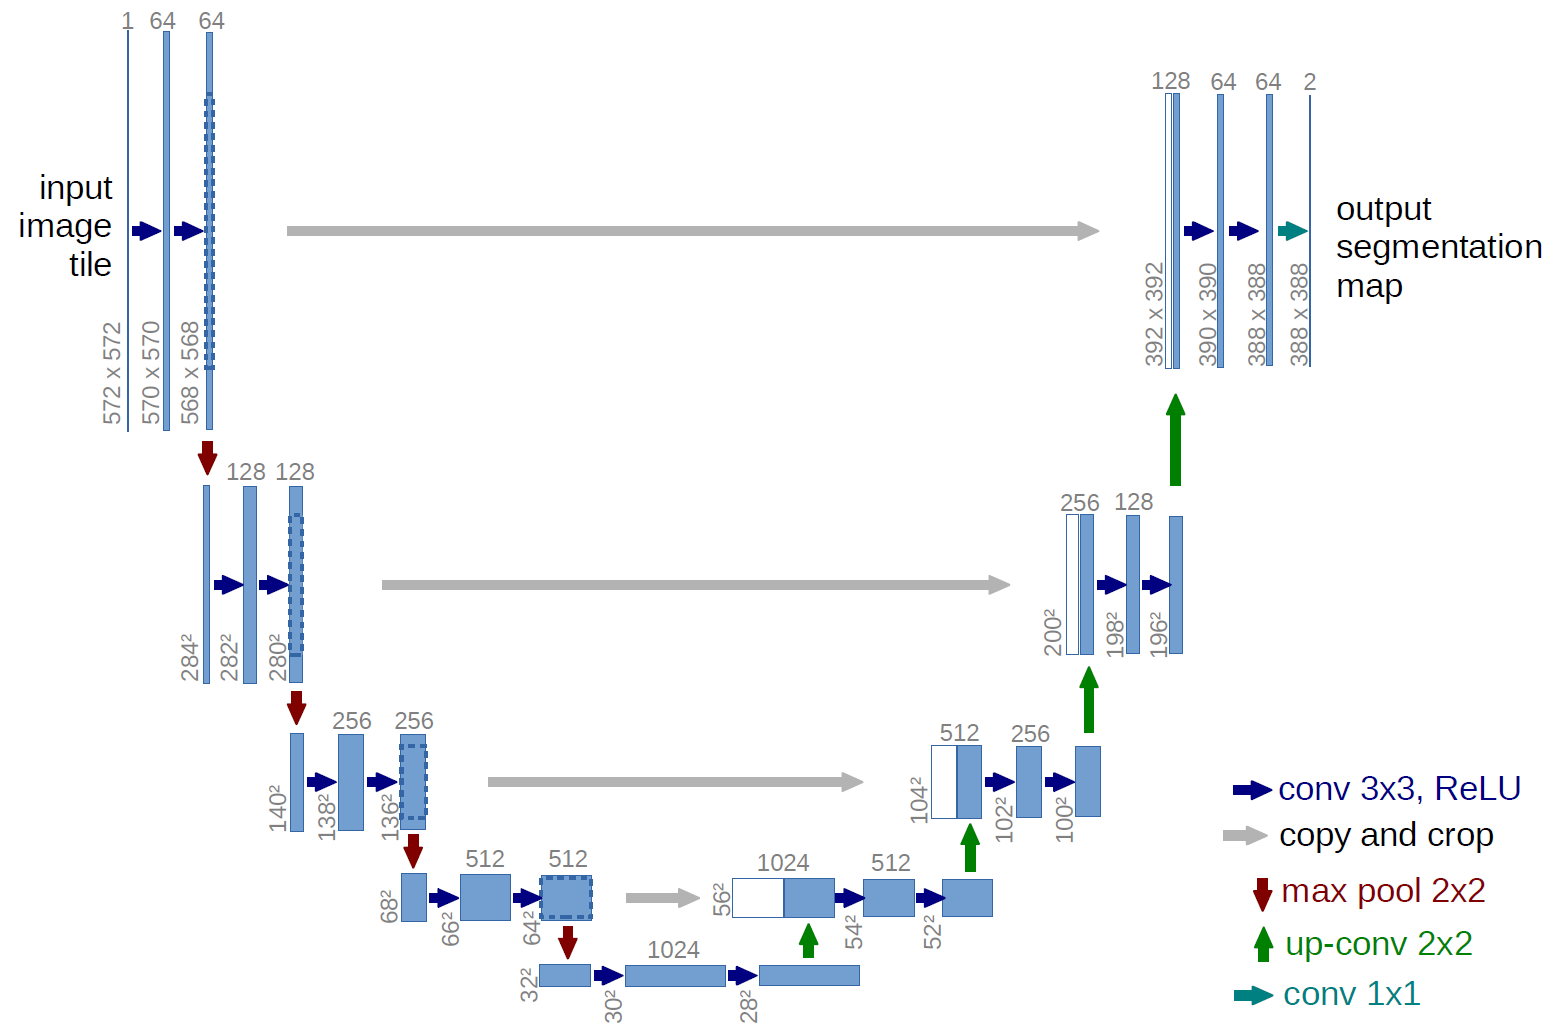
\includegraphics[width=0.8\textwidth]{static/unet_architecture.png}
\caption{UNet architecture.}
\label{fig:unet}
\end{figure}

\section{SRUNet Architecture}

SR-UNet is a deep convolutional neural network that is designed for super-resolution of images. Let's assume that we have a low-resolution input image \textbf{x} with spatial dimensions of W x H x C, where W and H represent the width and height of the image, and C is the number of channels. The goal is to generate a high-resolution output image \textbf{y} with spatial dimensions of W' x H' x C, where W' and H' are larger than W and H, respectively.

The SR-UNet model is composed of an encoder and a decoder, with skip connections between them. The encoder takes the input image \textbf{x} as input and applies a series of convolutional layers to reduce the dimensionality of the image and capture important features. The encoder can be represented as a function $f_\theta$ that takes the input image \textbf{x} and returns a feature map \textbf{f}:

$$ \textbf{f} = f_\theta(\textbf{x}) $$

The decoder takes the feature map \textbf{f} as input and applies a series of convolutional layers to upsample the image while preserving the details. The decoder can be represented as a function $g_\phi$ that takes the feature map \textbf{f} and returns the high-resolution output image \textbf{y}:

$$ \textbf{y} = g_\phi(\textbf{f}) $$

The skip connections are used to connect the corresponding encoder and decoder layers. Specifically, the feature maps from the encoder are concatenated with the feature maps from the corresponding decoder layers to help the model capture the fine-grained details and ensure that the output image is accurate.

In addition, the SR-UNet model uses residual blocks to help the model learn the difference between the low-resolution input image \textbf{x} and the high-resolution output image \textbf{y}. Each residual block consists of two convolutional layers and a shortcut connection that bypasses the convolutional layers. The output of the residual block can be expressed as:

$$ \textbf{z} = \textbf{x} + \textbf{W}_2\sigma(\textbf{W}_1\textbf{x}+\textbf{b}_1)+\textbf{b}_2 $$

where $\textbf{W}_1$ and $\textbf{W}_2$ are weight matrices, $\textbf{b}_1$ and $\textbf{b}_2$ are bias vectors, and $\sigma$ is the activation function.

% \begin{align}
% \text{L}{\text{total}} &= \alpha \text{L}{\text{LPIPS}} + \beta \text{L}{\text{SSIM}} \
% &= \alpha \frac{1}{N}\sum{i=1}^N d_{\text{LPIPS}}(\textbf{y}_i, \textbf{y}^i) + \beta \frac{1}{N}\sum{i=1}^N (1-\text{SSIM}(\textbf{y}_i, \textbf{y}^_i)),
% \end{align}

% where $\text{L}{\text{total}}$ is the total loss, $\text{L}{\text{LPIPS}}$ and $\text{L}_{\text{SSIM}}$ are the LPIPS and SSIM losses, respectively, and $\alpha$ and $\beta$ are the weighting coefficients for the two losses.

% $d_{\text{LPIPS}}(\textbf{y}_i, \textbf{y}^_i)$ represents the LPIPS distance between the predicted output image $\textbf{y}_i$ and the ground truth high-resolution image $\textbf{y}^_i$. LPIPS is a perceptual distance metric that measures the similarity between two images based on their perceptual features.

% $\text{SSIM}(\textbf{y}_i, \textbf{y}^_i)$ represents the structural similarity index between the predicted output image $\textbf{y}_i$ and the ground truth high-resolution image $\textbf{y}^_i$. SSIM is a popular image quality assessment metric that measures the structural similarity between two images based on their luminance, contrast, and structure.

% The values of $\alpha$ and $\beta$ can be adjusted to prioritize one loss over the other, depending on the specific requirements of the task. For example, if the goal is to prioritize perceptual quality, a higher value of $\alpha$ may be used to emphasize the LPIPS loss. Conversely, if the goal is to prioritize structural similarity, a higher value of $\beta$ may be used to emphasize the SSIM loss.

\Cref{fig:srunet} shows an high-level representation of the SRUNet architecture.

\begin{figure}[h]
\centering
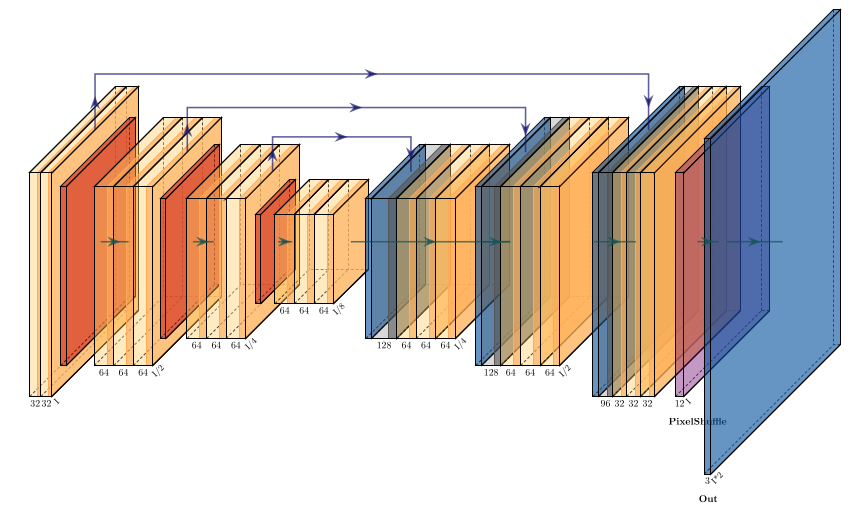
\includegraphics[width=0.8\textwidth]{static/srunet_architecture.png}
\caption{SRUNet architecture.}
\label{fig:srunet}
\end{figure}

\section{Training Setup}

To train the UNet and SRUNet models for super-resolution, we used a GAN framework with a combination of LPIPS and SSIM as the generator loss.

The GAN framework consists of a generator and a discriminator. The generator takes a low-resolution image as input and generates a high-resolution image. The discriminator takes either a low-resolution or a high-resolution image and outputs a probability score indicating whether the input image is real or fake.

The generator loss is composed of two parts: an adversarial loss and a content loss. The adversarial loss encourages the generator to generate images that are indistinguishable from real images, while the content loss encourages the generator to generate images that are similar to the target high-resolution images.

In this setup, we used LPIPS and SSIM as the content loss. LPIPS is a perceptual similarity metric that measures the distance between two images in terms of their perceptual features. SSIM is a structural similarity metric that measures the similarity between two images in terms of their structure, luminance, and contrast.

The generator loss can be represented as follows:

$$\mathcal{L}{G} = -\log(D(\hat{y})) + w{lips}\cdot LPIPS(\hat{y}, y_{gt}) + w_{ssim} \cdot (1 - SSIM(\hat{y}, y_{gt}))$$

where $\hat{y}$ is the generated high-resolution image, $y_{gt}$ is the ground truth high-resolution image, $D(\hat{y})$ is the probability score outputted by the discriminator for the generated image, $w_{lips}$ and $w_{ssim}$ are hyperparameters that control the relative importance of the LPIPS and SSIM losses, and $LPIPS$ and $SSIM$ are functions that compute the LPIPS and SSIM losses, respectively.

During training, we alternated between training the discriminator and training the generator. We used the Adam optimizer with a learning rate of 0.0002 for both the generator and discriminator. We also used gradient penalty regularization for the discriminator to ensure Lipschitz continuity.

% In this chapter, we discussed the architectures of the UNet and SRUNet models for super-resolution and the training setup using a GAN framework with LPIPS and SSIM as the generator loss. These models and techniques have been shown to be effective in improving the performance of super-resolution tasks in deep learning.

% UNet architecture
% 
% The UNet architecture was introduced by Ronneberger et al. in 2015 for biomedical image segmentation tasks. It has since been widely used for various image processing tasks, including super-resolution.
% 
% The UNet architecture consists of a contracting path and an expanding path. The contracting path is composed of a series of convolutional layers with max pooling layers in between. This path downsamples the input image to a lower resolution, while increasing the number of channels. The expanding path then upsamples the low-resolution feature map back to the original size of the input image, while decreasing the number of channels.
% 
% The expanding path also has skip connections that connect the corresponding feature maps from the contracting path to the expanding path. These skip connections help the model to preserve high-frequency information from the original input image.
% 
% Here is an illustration of the UNet architecture:
% 
% \section{SRUNet}
% \label{sec:srunet}
% 
% 
% SRUNet architecture
% 
% The SRUNet architecture was introduced by Tao et al. in 2017 for super-resolution tasks. It is an extension of the UNet architecture that includes residual blocks and dense connections.
% 
% The SRUNet architecture also has a contracting path and an expanding path, but each block in the expanding path is composed of a series of residual blocks with dense connections. Residual blocks consist of two convolutional layers with a skip connection that adds the input to the output of the second convolutional layer. Dense connections connect each layer to all subsequent layers in the same block.
% 
% Here is an illustration of the SRUNet architecture:
% 
% SRUNet architecture
% GAN training with LPIPS and SSIM as the generator loss
% 
% Now let's talk about setting up a GAN training using LPIPS and SSIM as the generator loss.
% 
% GANs consist of a generator and a discriminator. The generator takes a low-resolution image as input and generates a high-resolution image. The discriminator takes either a low-resolution or a high-resolution image and outputs a probability score indicating whether the input image is real or fake.
% 
% The goal of GAN training is to train the generator to generate high-quality images that are indistinguishable from real high-resolution images, while training the discriminator to accurately distinguish between real and fake images.
% 
% The generator loss is typically composed of two parts: an adversarial loss and a content loss. The adversarial loss encourages the generator to generate images that are indistinguishable from real images, while the content loss encourages the generator to generate images that are similar to the target high-resolution images.
% 
% In this setup, we will use LPIPS and SSIM as the content loss. LPIPS is a perceptual similarity metric that measures the distance between two images in terms of their perceptual features. SSIM is a structural similarity metric that measures the similarity between two images in terms of their structure and luminance.

% SRUNet: A Deep Learning-based Super-Resolution Model
% 
% In recent years, deep learning-based super-resolution models have achieved state-of-the-art performance in super-resolution tasks. One such model is SRUNet, which is an extension of the U-Net architecture. In this chapter, we will discuss the definition of SRUNet and how it differs from U-Net.
% 
% 3.1 Definition of SRUNet
% 
% SRUNet is a deep learning-based super-resolution model that uses a U-Net architecture with skip connections. The model takes a low-resolution image as input and generates a high-resolution image as output. The U-Net architecture is composed of an encoder and a decoder, with skip connections between them. The encoder consists of several convolutional layers that reduce the spatial resolution of the input image and increase its feature depth. The decoder consists of several deconvolutional layers that increase the spatial resolution of the feature maps and decrease their feature depth. Skip connections connect the encoder and decoder at each level, allowing the model to recover high-frequency details.
% 
% SRUNet extends the U-Net architecture by incorporating residual learning and dense connections. Residual learning allows the model to learn residual features between the low-resolution input and the high-resolution output. Dense connections allow the model to access the feature maps of all preceding layers, promoting information flow and feature reuse.
% 
% 3.2 Differences between SRUNet and U-Net
% 
% SRUNet differs from U-Net in several ways. First, SRUNet incorporates residual learning, allowing the model to learn residual features between the low-resolution input and the high-resolution output. This improves the ability of the model to capture high-frequency details and generate sharper images.
% 
% Second, SRUNet incorporates dense connections, allowing the model to access the feature maps of all preceding layers. This promotes information flow and feature reuse, improving the efficiency of the model and reducing the risk of vanishing gradients.
% 
% Third, SRUNet uses a depth-wise separable convolution in the bottleneck layer, reducing the number of parameters and improving the efficiency of the model. Depth-wise separable convolutions factorize a standard convolution into a depth-wise convolution and a point-wise convolution, reducing the computational cost of the operation.
% 
% Finally, SRUNet uses a residual scaling module in the output layer, which scales the residual features by a learnable parameter before adding them to the input image. This improves the stability of the model and reduces the risk of exploding gradients.
% 
% Overall, SRUNet improves upon the U-Net architecture by incorporating residual learning, dense connections, depth-wise separable convolutions, and a residual scaling module. These improvements lead to a more efficient and effective super-resolution model with state-of-the-art performance.
% 
% 3.3 Conclusion
% 
% In this chapter, we discussed SRUNet, a deep learning-based super-resolution model that uses a U-Net architecture with skip connections, residual learning, dense connections, depth-wise separable convolutions, and a residual scaling module. We also discussed the differences between SRUNet and U-Net, highlighting the improvements in efficiency and effectiveness provided by SRUNet. The discussion of SRUNet provides a foundation for the proposed work on optimizing deep learning models for visual quality improvement in super-resolution tasks.
% 
